% !TEX encoding = UTF-8 Unicode
% !TEX root = thesis-ex.tex
The FCal is a critical component in estimating the centrality of an event (See Section~\ref{sec:HICollisions} for an introduction to centrality).
While the direct measurement of the impact parameter is not possible, the centrality of an event directly correlates to number of reconstructed charged particles and the the energy deposited in the detector as shown in Figure~\ref{fig:nch_fcal}.
Thus, the energy deposited in the calorimeter can be used to estimate the centrality.
However, to avoid autocorrelations in the measurement, different detector regions are used for the analysis and the event classification.
Since the energy in the barrel region is directly correlated to the energy in the forward calorimeter as shown in Figure~\ref{fig:fcal_barrel}, event centrality can be determined using the transverse energy in the FCal, \ETfcal\.
The \ETfcal\. is divided in percentiles as shown in Figure~\ref{fig:fcal_distr}, with each bin corresponding to a centrality interval.
The 0--10\% centrality corresponds to most central collisions with the maximum overlap between the colliding nuclei, while the 90--100\% corresponds to the most peripheral collisions with the least overlap between the colliding nuclei.


 \begin{figure}
\centering
\begin{subfigure}{.45\textwidth}
  \centering
  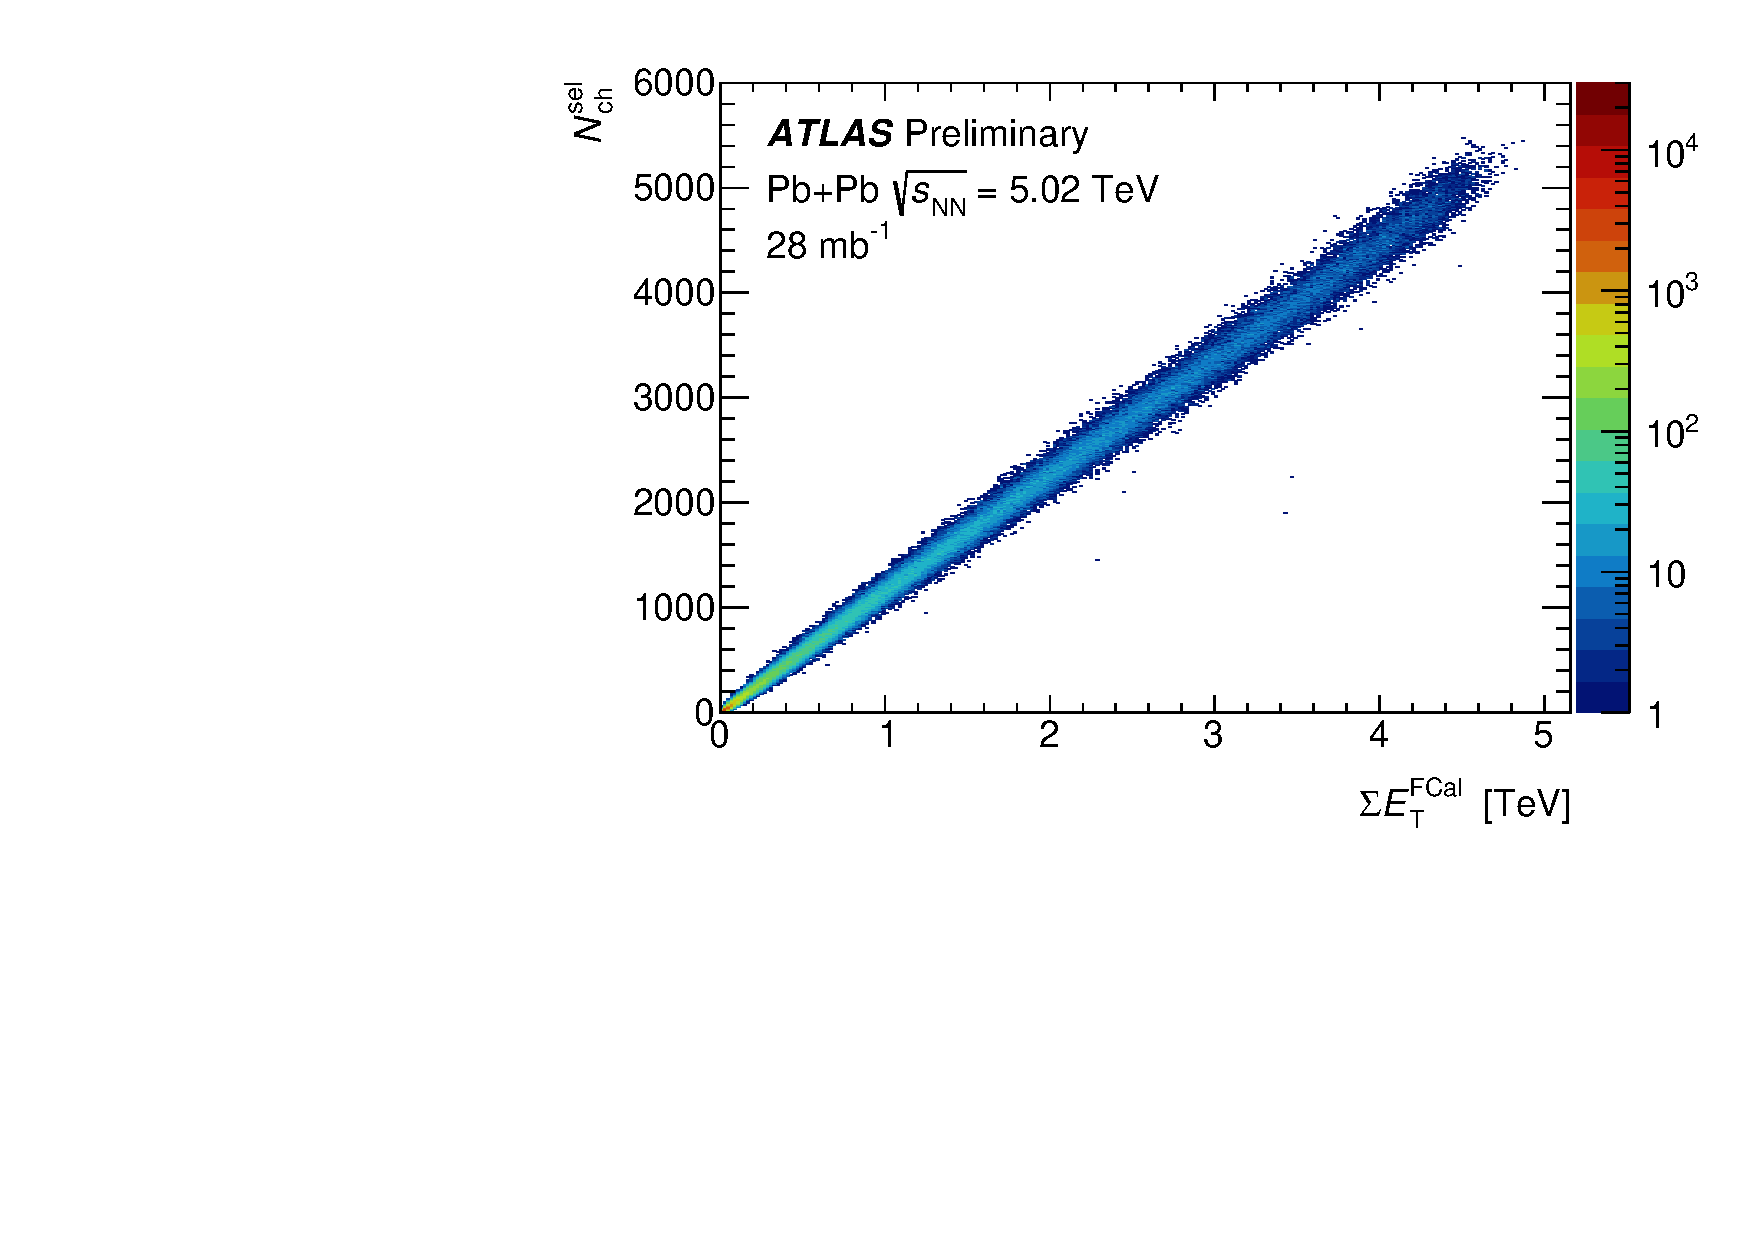
\includegraphics[width=\linewidth]{figures/setup/nch_fcal}
          \caption{}
          \label{fig:nch_fcal}
\end{subfigure}
\qquad  \qquad  
\begin{subfigure}{.45\textwidth}  
  \centering
  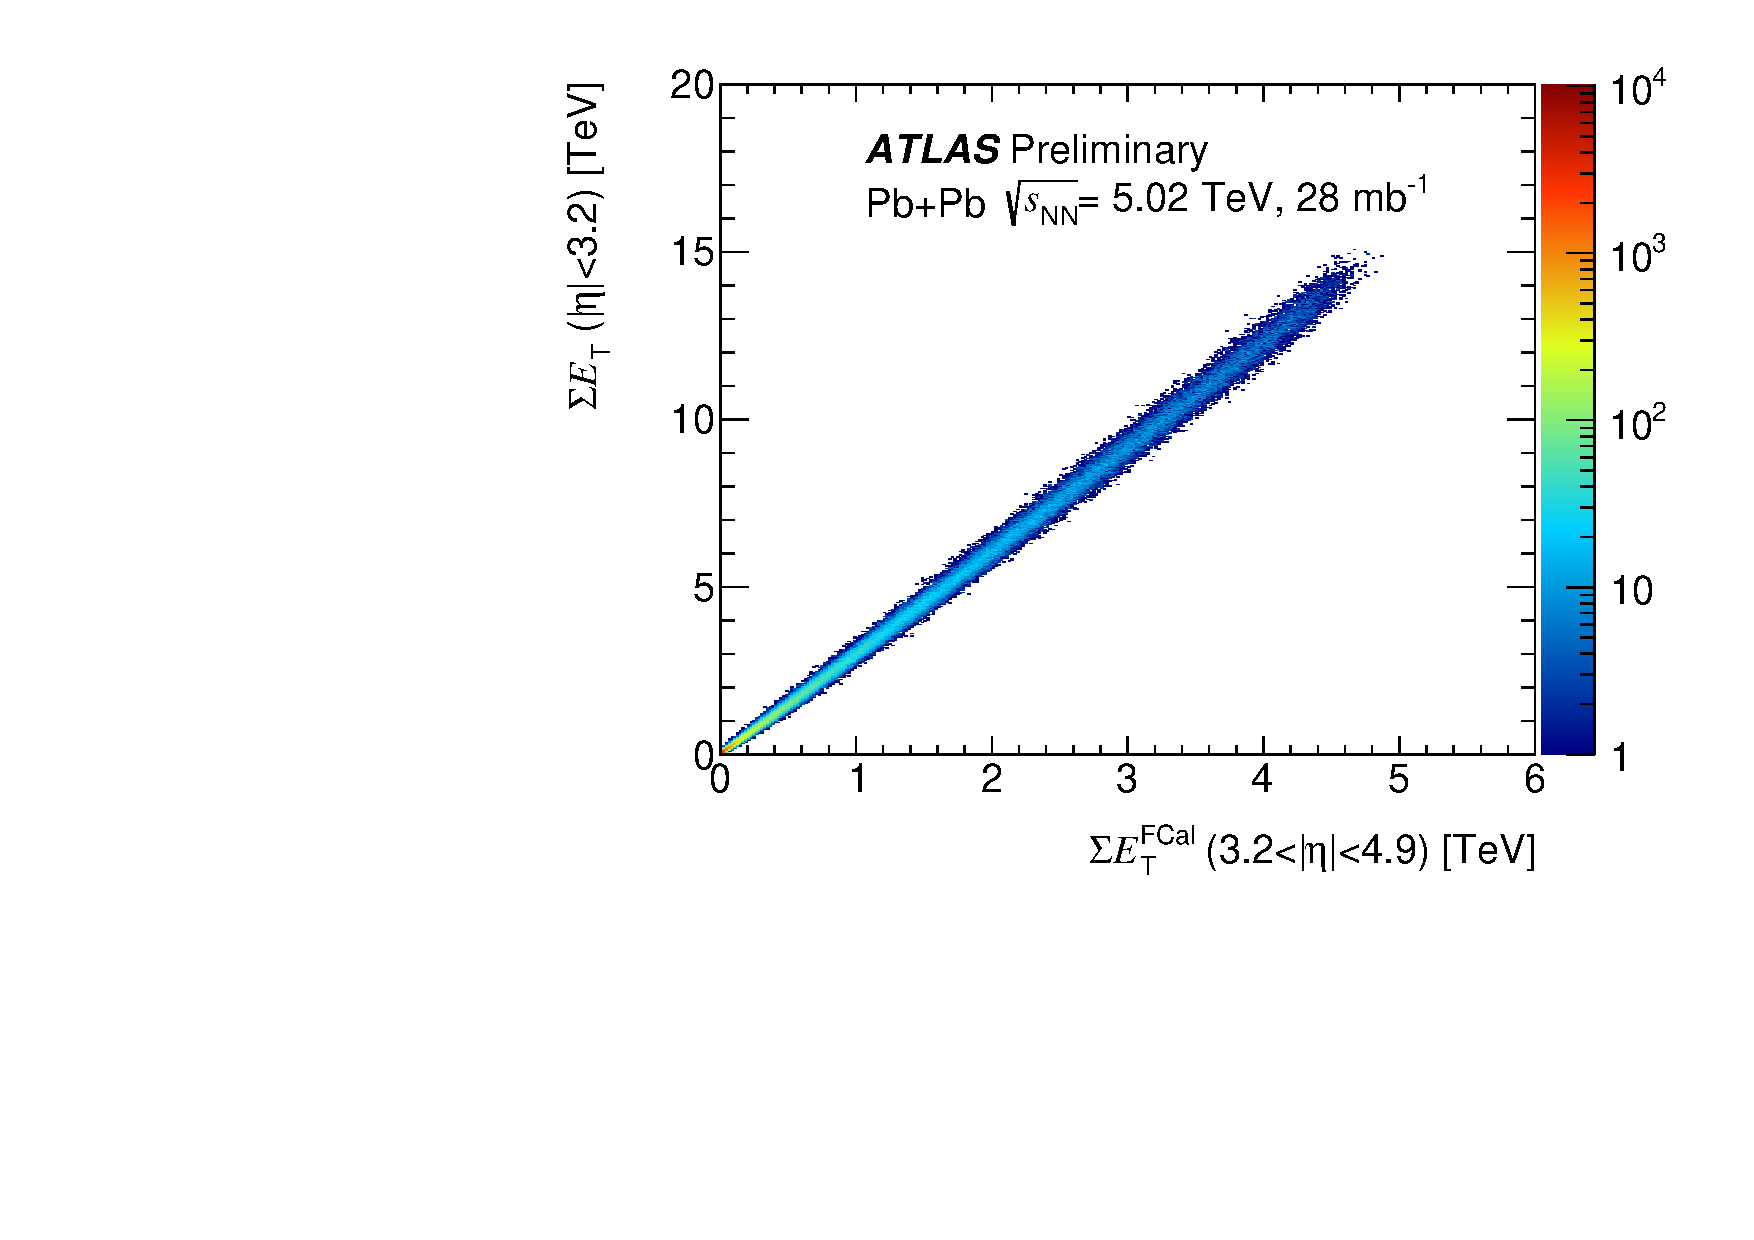
\includegraphics[width=\linewidth]{figures/setup/fcal_barrel}
          \caption{}
          \label{fig:fcal_barrel}
\end{subfigure}
\caption{(Left) Number of reconstructed charged particles $\Nch^{\rm sel}$ versus the total transverse energy in the FCal, \ETfcal.
(Right) Correlation of the total energy in the calorimeter in the interval of $|\eta| < 3.2$ with the total energy measured in the forward calorimeters.
Both plots are for \pbpb\ collisions with \sqrtsnn = 5.02 TeV.
Taken from Ref.~\cite{perfPlots}.}
\label{fig:jetcs}
\end{figure}



\begin{figure}[ht]
	\centering
        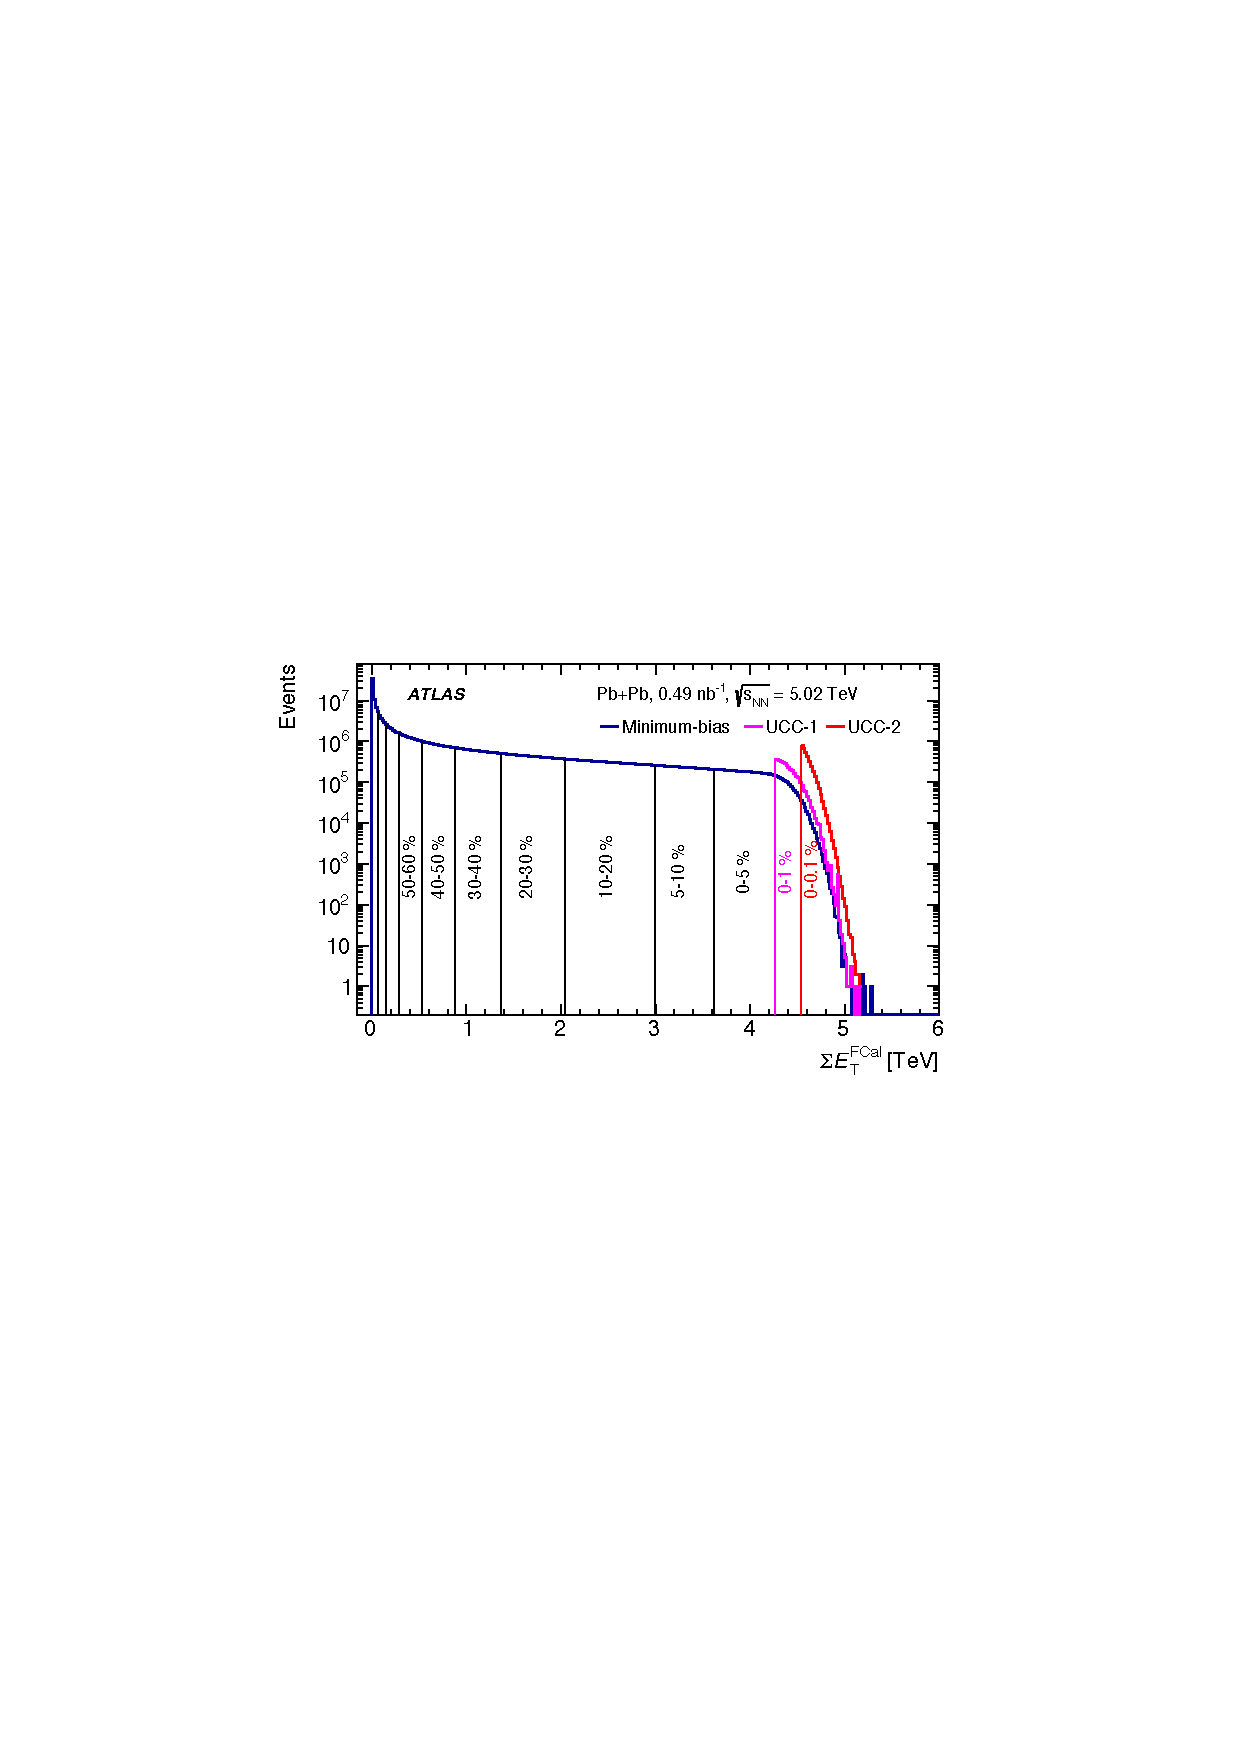
\includegraphics[width=0.5\textwidth]{figures/setup/fcal_distr}
          \caption{The \ETfcal\ distribution in $\sqrtsnn = 5.02$ TeV \pbpb\ collisions for events selected by the minimum bias trigger.
          The \ETfcal\ thresholds for several centrality intervals are marked with vertical lines and labelled on the plot.
           Also shown are the number of events over the 0--1\% and 0--0.1\% centrality intervals selected by the ultra-central triggers.
           Figure taken from Ref.~\cite{Aaboud:2018ves}.}
          \label{fig:fcal_distr}
\end{figure}
